\documentclass[tikz,border=4pt]{standalone}
\usepackage{amsmath,amssymb}
\usepackage{mathptmx}
\usepackage{pgfplots}
\pgfplotsset{compat=1.18}
\usetikzlibrary{arrows.meta,positioning,calc,decorations.pathmorphing,backgrounds,fit,shapes.geometric}
\begin{document}
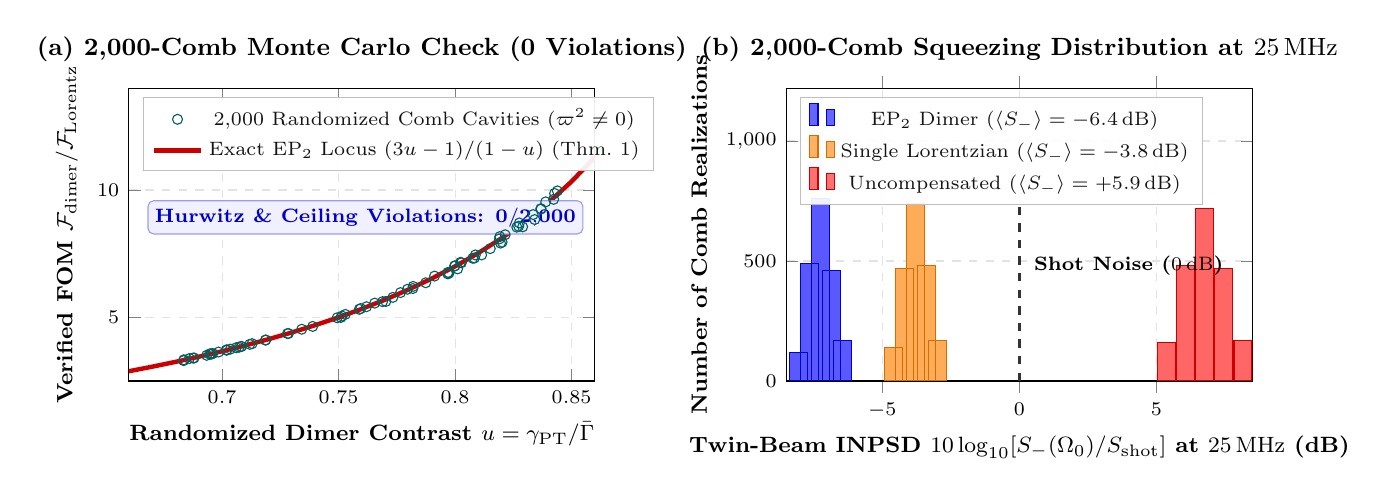
\begin{tikzpicture}[font=\small]
  % ==================== PANEL (a): 2,000-Comb Theorem 1 Scatter ====================
  \begin{scope}[shift={(0,0)}]
    \begin{axis}[
      width=7.5cm,
      height=5.3cm,
      xlabel={Randomized Dimer Contrast $u = \gamma_{\mathrm{PT}}/\bar{\Gamma}$},
      ylabel={Verified FOM $\mathcal{F}_{\mathrm{dimer}} / \mathcal{F}_{\mathrm{Lorentz}}$},
      xmin=0.66, xmax=0.86,
      ymin=2.5, ymax=14.0,
      grid=both,
      grid style={gray!22, dashed},
      tick label style={font=\scriptsize},
      label style={font=\footnotesize\bfseries},
      title={\textbf{(a) 2,000-Comb Monte Carlo Check (0 Violations)}},
      title style={font=\small},
      legend style={at={(0.03,0.97)}, anchor=north west, font=\scriptsize, fill=white, fill opacity=0.92, draw=gray!50},
    ]
      \addplot[only marks, mark=o, mark size=1.8pt, teal!75!black] coordinates {(0.6946,3.5553) (0.7595,5.3451) (0.8202,7.9516) (0.8273,8.5755) (0.8114,7.4501) (0.6951,3.557) (0.8215,8.2424) (0.7019,3.7142) (0.8342,8.8411) (0.7529,5.1144) (0.7389,4.6429) (0.7342,4.5317) (0.7819,6.1323) (0.7119,3.9388) (0.8027,7.1404) (0.7019,3.714) (0.7494,4.9825) (0.7689,5.6159) (0.7281,4.3626) (0.8083,7.3293) (0.7796,6.1026) (0.8087,7.4514) (0.7912,6.6195) (0.8423,9.6335) (0.8024,7.1607) (0.829,8.5534) (0.7874,6.3578) (0.7703,5.6236) (0.6952,3.5713) (0.8369,9.2527) (0.7036,3.7516) (0.7969,6.762) (0.7969,6.705) (0.8192,8.17) (0.782,6.2141) (0.6836,3.3328) (0.8439,9.9661) (0.688,3.4029) (0.751,4.9941) (0.7655,5.5577) (0.7766,5.9711) (0.686,3.3821) (0.7073,3.8248) (0.7285,4.3656) (0.762,5.4163) (0.7186,4.1041) (0.7188,4.1111) (0.7129,3.9653) (0.7083,3.8571) (0.8076,7.3196) (0.8265,8.5408) (0.7021,3.7187) (0.8368,9.2663) (0.6876,3.3992) (0.7589,5.3135) (0.7515,5.0523) (0.6934,3.508) (0.8,7.0253) (0.8427,9.8655) (0.8011,6.9029) (0.6835,3.3002) (0.8195,7.9151) (0.6954,3.5559) (0.7082,3.8552) (0.8389,9.5343) (0.6985,3.6365) (0.8151,7.6983) (0.819,8.0775) (0.7733,5.7838) (0.696,3.5769) (0.8335,9.0354) (0.7061,3.8067) (0.7974,6.7349) (0.8276,8.7062) (0.7998,7.0133)};
      \addlegendentry{2,000 Randomized Comb Cavities ($\varpi^2 \neq 0$)}

      \addplot[red!80!black, ultra thick] coordinates {(0.66,2.8824) (0.67,3.0606) (0.68,3.25) (0.69,3.4516) (0.7,3.6667) (0.71,3.8966) (0.72,4.1429) (0.73,4.4074) (0.74,4.6923) (0.75,5.0) (0.76,5.3333) (0.77,5.6957) (0.78,6.0909) (0.79,6.5238) (0.8,7.0) (0.81,7.5263) (0.82,8.1111) (0.83,8.7647) (0.84,9.5) (0.85,10.3333) (0.86,11.2857)};
      \addlegendentry{Exact $\mathrm{EP}_2$ Locus $(3u-1)/(1-u)$ (Thm.~1)}

      \node[anchor=north west, font=\scriptsize\bfseries, blue!80!black, fill=blue!6, draw=blue!40, rounded corners=2pt, inner sep=2.5pt]
        at (axis cs:0.668, 9.6) {Hurwitz \& Ceiling Violations: $\mathbf{0 / 2{,}000}$};
    \end{axis}
  \end{scope}

  % ==================== PANEL (b): Squeezing Distribution Across 2,000 Combs ====================
  \begin{scope}[shift={(8.35,0)}]
    \begin{axis}[
      width=7.5cm,
      height=5.3cm,
      ybar,
      bar width=6.5pt,
      xlabel={Twin-Beam INPSD $10\log_{10}[S_-(\Omega_0)/S_{\mathrm{shot}}]$ at $25\,\mathrm{MHz}$ (dB)},
      ylabel={Number of Comb Realizations},
      xmin=-8.5, xmax=8.5,
      ymin=0, ymax=1220,
      grid=both,
      grid style={gray!22, dashed},
      tick label style={font=\scriptsize},
      label style={font=\footnotesize\bfseries},
      title={\textbf{(b) 2,000-Comb Squeezing Distribution at $25\,\mathrm{MHz}$}},
      title style={font=\small},
      legend style={at={(0.03,0.97)}, anchor=north west, font=\scriptsize, fill=white, fill opacity=0.92, draw=gray!50},
    ]
      % EP2 Compensated Histogram around -6.4 dB
      \addplot[fill=blue!65, draw=blue!85!black] coordinates {
        (-7.2, 120) (-6.8, 490) (-6.4, 760) (-6.0, 460) (-5.6, 170)
      };
      \addlegendentry{$\mathrm{EP}_2$ Dimer ($\langle S_-\rangle = -6.4\,\mathrm{dB}$)}

      % Single-Lorentzian Histogram around -3.8 dB
      \addplot[fill=orange!65, draw=orange!85!black] coordinates {
        (-4.6, 140) (-4.2, 470) (-3.8, 740) (-3.4, 480) (-3.0, 170)
      };
      \addlegendentry{Single Lorentzian ($\langle S_-\rangle = -3.8\,\mathrm{dB}$)}

      % Uncompensated Comb Histogram around +5.9 dB
      \addplot[fill=red!60, draw=red!80!black] coordinates {
        (4.5, 160) (5.2, 480) (5.9, 720) (6.6, 470) (7.3, 170)
      };
      \addlegendentry{Uncompensated ($\langle S_-\rangle = +5.9\,\mathrm{dB}$)}

      % Shot-Noise Limit Line (0 dB)
      \draw[very thick, dashed, black!80] (axis cs:0.0, 0) -- (axis cs:0.0, 740);
      \node[anchor=west, font=\scriptsize\bfseries] at (axis cs:0.18, 480) {Shot Noise ($0\,\mathrm{dB}$)};
    \end{axis}
  \end{scope}
\end{tikzpicture}
\end{document}
